\begin{comment}
comment from Manoj
Start with the properties of microservices and not directly Granularity? May be if we had talked about the qualities of microservices, it would have made more sense.
comment from Andrea
- compare the 'dimension by interface' and 'dimension by realization', and provide which should be considered
- define efficiency and reuse efficiency
- create a table to show what are good and bad services vs your goal and case.
- use common understandable term for 'volume' of service, either 'size'
To be done
- factors influencing size of a service such as single responsibility principle, technology, bounded context, autonomy
\end{comment}

\chapter{Granularity}\label{chapter:granularity}
In this chapter, a detailed concept regarding size of microservices will be discussed. A major focus would be to research various qualitative aspects of granularity of microservices. The section \ref{section:granularity/principles} lists various principles which can guide to model correct size considering various important aspects. Later, in section \ref{section:granularity/dimensions}, various interpretations defining dimensions of microservices are presented. Finally, the secion provides a complete picture of various factors which determine granularity.

\section{Introduction}\label{section:granularity/introduction}
The granularity of a service is often ambiguous and has different interpretation. In simple term, it refers to the size of the service. However, the size itself can be vague. It can neither be defined as a single quantitative value nor it can be defined in terms of single dependent criterion. It is difficult to define granularity in terms of number because the concepts defining granularity are vague and subjective in nature. If we choose an activity supported by the service to determine its granularity then we cannot have one fixed value instead a hierarchical list of answers; where an activity can either refer to a simple state change, any action performed by an actor or a complete business process. \cite{Linthicum:2015aa}, \cite{Raf-Haesen:2015aa}
\\
Although, the interest upon the granularity of a component or service for the business users only depends upon their business value, there is no doubt that the granularity affects the architecture of a system. The honest granularity of a service should reflect upon both business perspective and should also consider the impact upon the overall architecture.
\\
If we consider other units of software application, we come from object oriented to component based and then to service oriented development. Such a transistion has been considered with the increase in size of the individual unit. The increase in size is contributed by the interpretation or the choice of the abstraction used. For example, in case of object oriented paradigm, the abstraction is chosen to represent close impression of real world objects, each unit representing fine grained abstraction with some attributes and functionalities. 
\\
Such abstraction is a good approach towards development simplicity and understanding, however it is not sufficient when high order business goals have to be implemented. It indicates the necessity of coarser-grained units than units of object oriented paradigm. Moreover, component based development introduced the concept of business components which target the business problems and are coarser grained. The services provide access to application where each application is composed of various component services. \cite{Linthicum:2015aa}

\section{Basic Principles to Service Granularity}\label{section:granularity/principles}
In addition to quantitative perspective on granularity, it can be helpful to approach the granularity qualitatively. The points below are some basic principls derived from various scientific and research papers, which attempt to define the qualitative properties of granularity. Hopefully, these principles will be helpful to come with the service of right granularity.

\begin{enumerate}
\item The correct granularity of a component or a service is dependent upon the time. The various supporting technologies that evolve during time can also be an important factor to define the level of vertical decomposition. For eg: with the improvement in virtualization, containerization as well as platform as a service technologies, it is fast and easy for deployment automation which supports multiple fine-grained services creation.\cite{Peter-Herzum:2000aa}

\item A good candidate for a service should be independent upon the implementation but should depend upon the understandability of domain experts.

\cite{Raf-Haesen:2015aa, Peter-Herzum:2000aa}
\item A service should be an autonomous reusable component and should support various cohesion such as functional (group similar functions), temporal(change in the service should not affect other services), run-time(allocate similar runtime environment for similar jobs; eg. provide same address space for jobs of similar computing intensity) and actor (a component should provide service to similar users).
\cite{Raf-Haesen:2015aa}, \cite{Peter-Herzum:2000aa}

\item A service should not support huge number of operations. If it happens, it will affect high number of customers on any change and there will be no unified view on the functionality. Furthermore, if the interface of the service is small, it will be easy to maintain and understand.\cite{Raf-Haesen:2015aa}, \cite{Pierre-Reldin:2007aa}

\item A service should provide transaction integrity and compensation. The activities supported by a service should be within the scope of one transaction. Additionally, the compensation should be provided when the transaction fails. If each operation provided by the service map to one transaction, then it will improve availability and fault-recovery. \cite{Raf-Haesen:2015aa}, \cite{Foody:2005aa} \cite{Bianco:2007aa}

\item The notion of right granularity is more important than that of fine or coarse. It depends upon the usage condition and moreover is about balancing various qualities such as reusability, network usage, completeness of context etc. \cite{Raf-Haesen:2015aa}, \cite{Lawrence-Wilkes:2004aa}

\item The level of abstraction of the services should reflect the real world business activities. Doing so will help to map business requirements and technical capabilities. \cite{Pierre-Reldin:2007aa}

\item If there are ordering dependencies between the operations, it will be easy to implement and test if the dependent operations are all combined into a single service. \cite{Bianco:2007aa}

\item There can be two better approaches for breaking down an abstraction. One way is to separate redundant data or data with different semanting meaning. The other approach is to divide services with limited control and scope. For example: A Customer Enrollment service which deals with registration of new customers and assignment of unique customer ID can be divided into two independent fine-grained services: Customer Registration and ID Generation, each service will have limited scope and separate context of Customer.\cite{Pierre-Reldin:2007aa}

\item If there are functionalities provided by a service which are more likely to change than other functionalities. It is better to separate the functionality into a fine-grained service so that any further change on the functionality will affect only limited number of consumers. \cite{Bianco:2007aa}
 
\end{enumerate}

\section{Dimensions of Granularity}\label{section:granularity/dimensions}
As already mentioned in \ref{section:granularity/introduction}, it is not easy to define granularity of a service quantitatively. However, it can be made easier to visualize granularity if we can project it along various dimensions, where each dimension is a qualifying attribute responsible for illustrating size of a service. Eventhough the  dimensions discussed in this section will not give the precise quantity to identify granularity, it will definitely give the hint to locate the service in granularity space. It will be possible to compare the granularity of two distinct services. Moreover, it will be interesting and beneficial to know how these dimensions relate to each other to define the size.

\subsection{Dimension by Interface}\label{subsection:granularity/dimensions/interface}
One way to define granularity is by the perception of the service interface as made by its consumer. The various properties of a service interface responsible to define its size are listed below.
\begin{enumerate}
\item Functionality: It qualifies the amount of functionality offered by the service. The functionality can be either default functionality, which means some basic group of logic or operation provided in every case. Or the functionality can be parameterized and depending upon some values, it can be optionally provided. Depending upon the functionality volume, the service can be either fine-grained or course-grained than other service. Considering functionality criterion, A service offering basic CRUD functionality is fine-grained than a service which is offers some accumulated data using orchestration. \cite{Raf-Haesen:2015aa}
\\
\item Data: It refers to the amount of data handled or exchanged by the service. The data granularity can be of two types. The first one is input data granularity, which is the amount of data consumed or needed by the service in order to accomplish its tasks. And the other one is ouput data granularity, which is the amount of data returned by the service to its consumer. Depending upon the size and quantity of business object/objects consumed or returned by the service interface, it can be coarse or fine grained. Additionally, if the business object consumed is composed of other objects rather than primitive types, then it is coarser-grained. For example: the endpoint "PUT customers/C1234" is coarse-grained than the endpoint "PUT customers/C1234/Addresses/default" because of the size of data object expected by the service interface. \cite{Raf-Haesen:2015aa}
\\
\item Business Value: According to \cite{Rolland:2015aa}, each service is associated with an intention or business goal and follows some strategy to achiee that goal. The extent or magnitude of the intention can be perceived as a metric to define granularity. A service can be either atomic or aggregate of other services which depends upon the level of composition directly influenced by the extent of target business goal. An atomic service will have lower granularity than an aggregate in terms of business value. For example, sellProduct is coase-grained than acceptPayment, which is again coarse-grained than validateAccountNumber. \cite{Raf-Haesen:2015aa}
\end{enumerate}

\subsection{Dimension by Interface Realization}\label{subsection:granularity/dimensions/interface_realization}
The section \ref{subsection:granularity/dimensions/interface} provides the aspect of granularity with respect to the perception of customer to interface. However, there can be different opinion regarding the same properties, when it is viewed regarding the imlementation. This section takes the same aspects of granularity and try to analyze them when the services are implemented.
\begin{enumerate}
\item Functionality: In section \ref{subsection:granularity/dimensions/interface}, it was mentioned that an orchestration service has higher granularity than its constituent services with regard to default functionality. If the realization effort is focused, it may only include compositional and/or compensation logic because the individual tasks are acomplshed by the constituent service interfaces. Thus, in terms of the effort in realizing the service it is fine-grained than from the view point of interface by consumer. \cite{Raf-Haesen:2015aa}
\\
\item Data: In some cases, services may utilize standard message format. For example: financial services may use \acrshort{SWIFT} for exchanging finanicial messages. These messages are extensible and are coarse grained in itself. However, all the data accepted by the service along with the message may not be required and used in order to fulfil the business goal of the service. In that sense, the service is coarse-grained from the viewpoint of consumer but is fine-grained in realization point of view. \cite{Raf-Haesen:2015aa}
\\
\item Business Value: It can make a huge impact when analyzing business value of service if the realization of the service is not considered well. For example: if we consider data management interface which supports storage, retrieval and transaction of data, it can be considered as fine-grained because it will not directly impact the business goals. However, since other services are very dependent in its performance, it becomes necessary to analyse the complexity associated with the implementation, reliablity and change the infrastructure if needed. These comes with additional costs, which should well be analyzed. From the realization point of view, the data service is coarse-grained than its view by consumer. \cite{Raf-Haesen:2015aa}
\end{enumerate}

\begin{framed}
\textbf{\textit{Principle: A high Functionality granularity does not necessarily mean high business value granularity}}
\\
It may seem to have direct proportional relationship between functionality and business value granularity. The business value of a service reflects business goals however the functionality refers to the amount of work done by the service. A service to show customer history can be considered to have high functionality granularity because of the involved time period and database query. However, it is of very low business value to the enterprise. \cite{Raf-Haesen:2015aa}
\end{framed}


\subsection{R\textsuperscript{3} Dimension}\label{subsection:granularity/dimensions/r3}
Keen \cite{Keen:2015aa} and later  Weill and Broadbent \cite{Weill:1998aa} introduced a separate group of criteria to measure granularity of service. The granularity was evaluated in terms of two dimensions as shown in the Figure \ref{fig:Reach-Range Model}

\begin{figure}[H]
\begin{center}
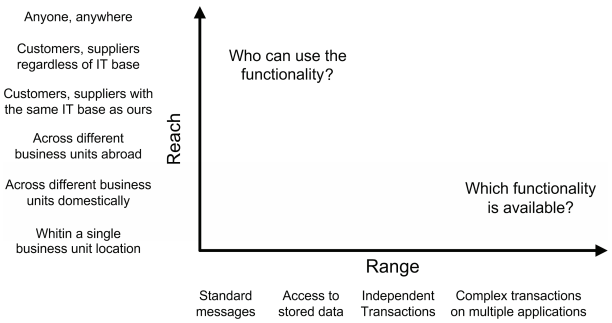
\includegraphics[width=0.8\textwidth]{figures/Granularity-R3-one}
\caption{Reach and Range model from \cite{Keen:2015aa, Weill:1998aa}}
\label{fig:Reach-Range Model}
\end{center}
\end{figure}

Reach: It provides various levels to answer the question “Who can use the functionality? ”.  It provides the extent of consumers, who can access the functionality provide  by the service. It can be a customer, the customers within an organization, supplier etc. as given by the Figure \ref{fig:Reach-Range Model}.
\\
Range: It gives answer to “Which functionality is available? ”. It shows the extent to which the information can be accessed from or shared with the service. The levels of information accessed are analyzed depending upon the kind of business activities accessible from the service. It can be a simple data access, a transaction, message transfer etc as shown in the Figure \ref{fig:Reach-Range Model} The 'Range' measures the amount of data exchanged in terms of the levels of business activities important for the organization. One example for such levels of activities with varying level of 'Range' is shown in Figure \ref{fig:Range Example}.
\begin{figure}[H]
\begin{center}
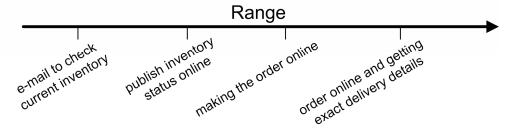
\includegraphics[width=0.8\textwidth]{figures/Granularity-R3-two}
\caption{Example to show varying Range from \cite{Keen:2015aa, Weill:1998aa}}
\label{fig:Range Example}
\end{center}
\end{figure}
In the figure \ref{fig:Range Example}, the level of granularity increases as the functionality moves from 'accessing e-mail message' to 'publishing status online' and then to 'creating order'. It is due to the change in the amount of data access involved in each kind of functionality. Thus, the 'Range' directly depends upon the range of data access.
\\
As the service grows,  alongside 'Reach' and 'Range' also peaks up, which means the extent of consumers as well as the kind of functionality increase. This will add complexity in the service. The solution proposed by \cite{Cockburn:2001aa} is to divide the architecture into services. However, only 'Reach' and 'Range' will not be enough to define the service. It will be equally important to determine scope of the individual services. The functionality of the service then should be define in two distinct dimensions 'which kind of functionality' and 'how much functionality'. This leads to another dimension of service as described below.
\cite{Keen:2015aa, Weill:1998aa, Pierre-Reldin:2007aa}
\\
Realm: It tries to create a boundary around the scope of the functionality provided by the service and thus clarifies the ambiguity created by 'Range'. If we take the same example as given by Figure \ref{fig: Range Example}, the range alone defining the kind of functionaly such as creating online order does not explicitly clarifies about what kind of order is under consideration. The order can be customer order or sales order. The specification of 'Realm' defining what kind of order plays role here. So, we can have two different services each with same 'Reach' and 'Range' however different 'Realm' for customer order and Sales order.  \cite{Keen:2015aa, Weill:1998aa, Pierre-Reldin:2007aa}

The consideration of all aspects of a service including 'Reach', 'Range' and 'Realm' give us a model to define granularity of a service and is called R\textsuperscript{3} model. The volume in the R\textsuperscript{3} space for a service gives its granularity. A coarse-grained service has higher R\textsuperscript{3} volume then fine-grained service. The figures \ref{fig:R3 volume-granularity analogy greater}  and \ref{fig:R3 volume-granularity analogy equal} show such volume-granularity analogy given by R\textsuperscript{3} model. \cite{Keen:2015aa, Weill:1998aa, Pierre-Reldin:2007aa}

\begin{figure}[H]
\begin{center}
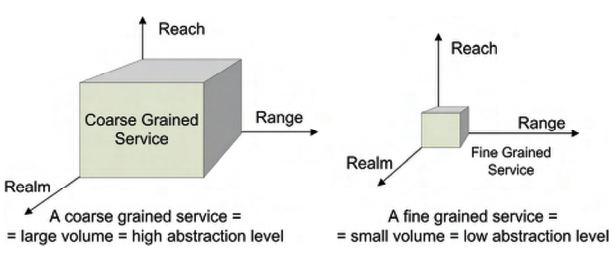
\includegraphics[width=0.8\textwidth]{figures/Granularity-R3-three}
\caption{R\textsuperscript{3} Volume-Granularity Analogy to show direct dependence of granularity and volume \cite{Pierre-Reldin:2007aa}}
\label{fig:R3 volume-granularity analogy greater }
\end{center}
\end{figure}

\begin{figure}[H]
\begin{center}
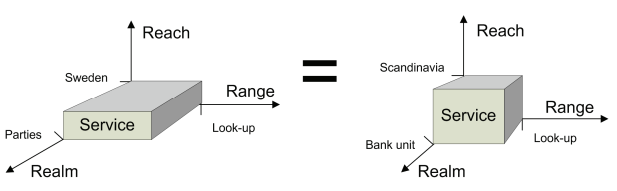
\includegraphics[width=0.8\textwidth]{figures/Granularity-R3-four}
\caption{R\textsuperscript{3} Volume-Granularity Analogy to show same granularity with different dimension along axes \cite{Pierre-Reldin:2007aa}}
\label{fig:R3 volume-granularity analogy equal}
\end{center}
\end{figure}


\subsection{Retrospective}\label{subsection:granularity/dimensions/retrospective}
The sections \ref{subsection:granularity/dimensions/interface} and \ref{subsection:granularity/dimensions/interface_realization} classified granularity of a service along three different directions: data, functionality and business value. Moreover, the interpretation from the viewpoint of interface by consumer and the viewpoint of producer for realization were also made.
Again, the section \ref{subsection:granularity/dimensions/r3} divides the aspect of granularity along Reach, Range and Realm space, the granularity given by the volume in the R\textsuperscript{3} space.
Despite of good explanation regarding each aspect, the classification along data, functionality and business value do not provide discrete metrics to define granularity in terms of quantitatively. However, the given explanations and criteria are well rounded to compare two different services regarding granularity. These can be effectively used to classify if a service is fine-grained than other service.
The R\textsuperscript{3} model in section \ref{subsection:granularity/dimensions/r3} additionally provides various levels of granularity along each axis. This makes it easy to at least measure the granularity and provides flexibility to compare the granularity between various services.
\\
A case study \cite{Pierre-Reldin:2007aa} using data, functionality and business criteria to evaluate the impact of granularity on the complexity in the architecture is held. The study was done at KBC Bank & Insurance Group of central Europe. Along the study, the impact of each kind of granularity is verified. The important results fromt the study are listed below.

\begin{enumerate}
\item A coarse-grained service in terms of 'Input Data' provides better transactional support, little communication overhead and also helps in scalability. However, there is a chance of data getting out-of-date quickly.
\item A coarse-grained service in terms of 'Output Data' also provides good communication efficiency and supports reusability.
\item A fine-grained service along 'Default Functionality' has high reusability and stability but low reuse efficiency.
\item A coarse-grained service due to more optional functionalities has high reuse efficiency, high reusability and also high stability but the implementation or realization is complicated.
\item A coarse-grained service along 'Business Value' has high consumer satisfaction value and emphasize the architecturally crucial points fulfilling business goals.
\end{enumerate}

Similarly, a study was carried out in Handelsbanken in sweden, which has been working with Service-Oriented architecture. The purpose of the study was to analyze the impact of R\textsuperscript{3} model on the architecture. It is observed that there are different categories of functionalities essential for an organization. Some functionality can have high Reach and Range with single functionality and other may have complex functionality with low Reach and Range. The categorization and realization of such functionalities should be accessed individually. It is not necessary to have same level of granularity across all services or there is no one right volume for all services. However, if there are many services with low volume, then we will need many services to accomplish a high level functionality. Additionally, it will increase interdependency among services and network complexity. Finally, the choice of granularity is completely dependent upon the IT-infrastructure of the company. The IT infrastructure decides which level of granularity it can support and how many of them. \cite{Pierre-Reldin:2007aa}


\begin{framed}
\textbf{\textit{Principle: IT-infrastructure of an organization affects granularity.}} \label{principle:granularity/IT_infrastructure}
\\
The right value of granularity for an organization is highly influenced by its IT infrastructure. The organization should be capable of handling the complexities such as communication, runtime, infrastructure etc if they choose low granularity. \cite{Pierre-Reldin:2007aa}
\end{framed}

Additionally, it is observed that a single service can be divided into number of granular services by dividing across either Reach, Range or Realm. The basic idea is to make the volume as low as possible as long as it can be supported by IT-infrastructure. Similarly, each dimension is not completely independent from other. For example: If the reach of a service has to be increased from domestic to global in an organization then the realm of the functionality has to be decreased in order to make the volume as low as possible, keep the development and runtime complexities in check. \cite{Pierre-Reldin:2007aa}

\begin{framed}
\textbf{\textit{Principle: Keep the volume low if possible.}}
\\
If supported by IT-infrastructure, it is recommended to keep the volume of service as low as possible, which can be achieved by managing the values of Reach, Range and Realm. It will help to decrease development and maintenance overload. \cite{Pierre-Reldin:2007aa}
\end{framed}

\section{Problem Statement}\label{section:granularity/problem_statement}
This chapter analysed various qualitative aspects related to granularity of microservices. The interesting thing to notice is various dimensions of size across data, functionality and business value. But it is also necessary to look into it in quantitative approach. Also, the various principles listed in section \ref{section:granularity/principles} points to other qualities of microservices except granularity. The granularity is not only attribute which is important while modeling microservices but there are other quality attributes which affect granularity and influence on the quality of microservices. The next task will be to study various other quality attributes affecting microservices and derive their quantitative metrices.

\begin{comment}
An additional contribution to defining the granularity has been made when the differentiating features of distributed system are taken into consideration. The granularity of a service depends upon the coupling and cohesion. In order to find the right granularity for a service, we need to balance between coupling and cohesion.
The coupling can be determined from the dependency graph between a service and its consumers. The goal is to minimize the coupling of individual service and to the application as a whole.
The cohesion is evaluated by the likeliness of the operations supported by the service. It considers that higher the similarities among the operations, higher the cohesion is.  \cite{Xiao-jun:2015aa}, \cite{Mikhail-Perepletchikov:2015aa}, \cite{Bingu-Shim:2008aa}

Service Hierarchy
\end{comment}

 